
\begin{center}
    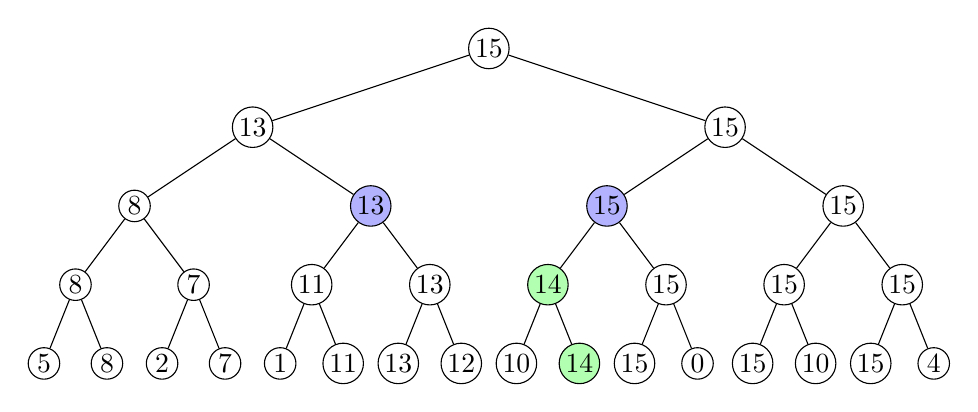
\begin{tikzpicture}[
        level distance=1cm,
        sibling distance=0pt,
        every node/.style = {circle, draw, minimum size=4mm, inner sep=1pt},
        level 1/.style={sibling distance=6cm},
        level 2/.style={sibling distance=3cm},
        level 3/.style={sibling distance=1.5cm},
        level 4/.style={sibling distance=0.8cm},
        level 5/.style={sibling distance=0.5cm}
      ]
      
      \node {15}
      child {node {13}
        child {node {8}
          child {node {8}
            child {node {5}}
            child {node {8}}
          }
          child {node {7}
            child {node {2}}
            child {node {7}}
          }
        }
        child {node[fill=blue!30] {13}
          child {node {11}
            child {node {1}}
            child {node {11}}
          }
          child {node {13}
            child {node {13}}
            child {node {12}}
          }
        }
      }
      child {node {15}
        child {node[fill=blue!30] {15}
          child {node[fill=green!30] {14}
            child {node {10}}
            child {node[fill=green!30] {14}}
          }
          child {node {15}
            child {node {15}}
            child {node {0}}
          }
        }
        child {node {15}
          child {node {15}
            child {node {15}}
            child {node {10}}
          }
          child {node {15}
            child {node {15}}
            child {node {4}}
          }
        }
      };
      
      \end{tikzpicture}
\end{center}
